\section{TAREA 2: CREAMOS NUESTRO PRIMER PAQUETE DTSX}

\begin{enumerate}
    \item Crear un proecto de Business Intelligense : Integration Services
     \begin{center}
            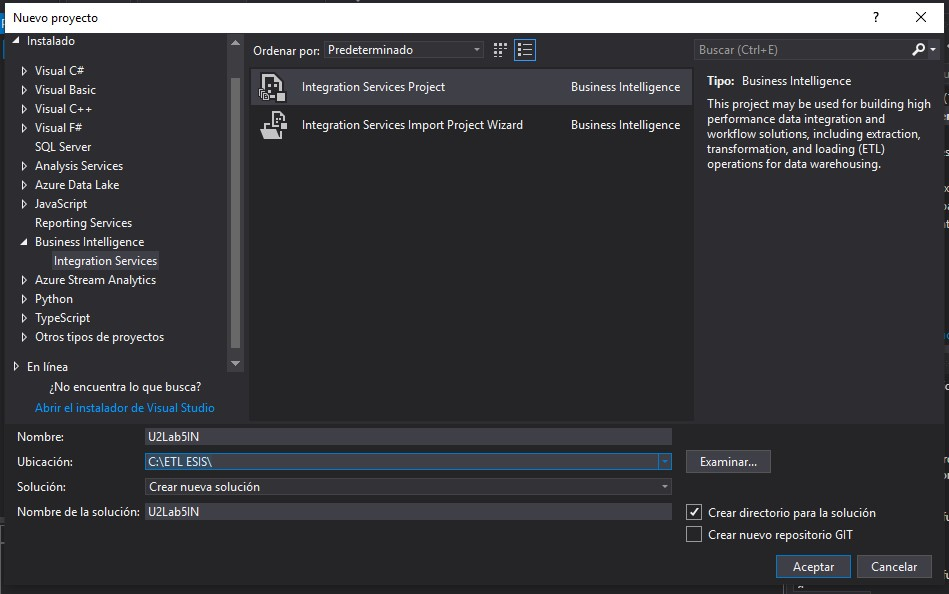
\includegraphics[width=10cm]{imagenes/bi_1.jpg}
        \end{center}
        
    \item Agregamos el paquete Import01.dtsx generado anteriormente
     \begin{center}
            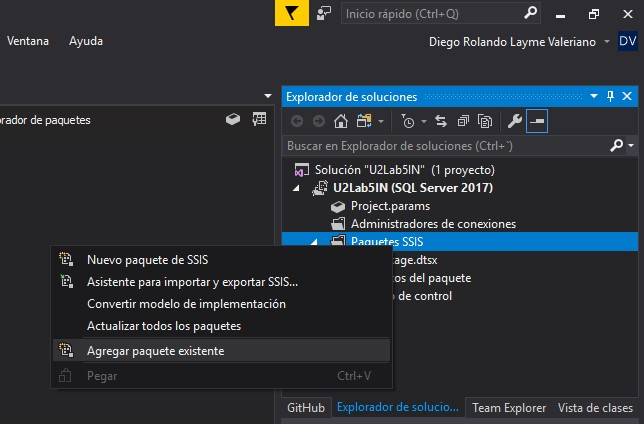
\includegraphics[width=10cm]{imagenes/bi_2.jpg}
        \end{center}
        
        
                
    \item Configuramos una nueva conexion 
     \begin{center}
            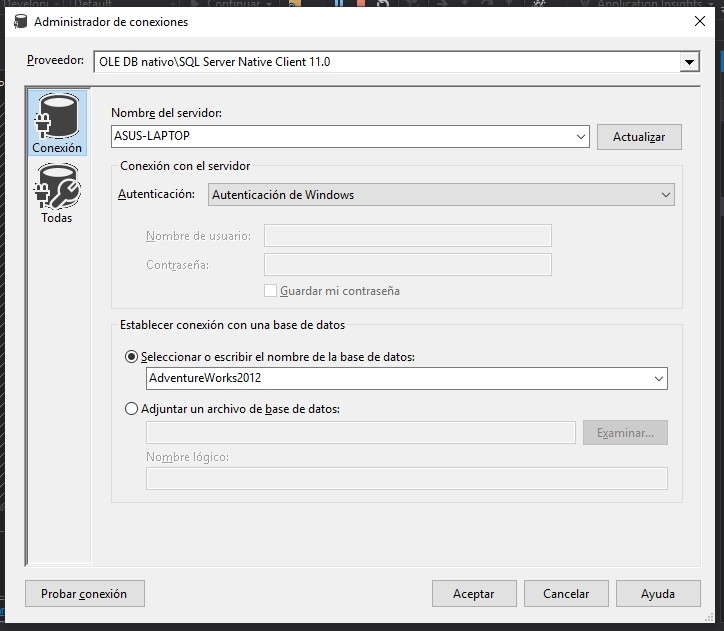
\includegraphics[width=10cm]{imagenes/registros_2_conexion.jpg}
        \end{center}
        
   \item Agregamos una Tarea de flujo de datos y  una tarea de Ejecutar SQL
     \begin{center}
            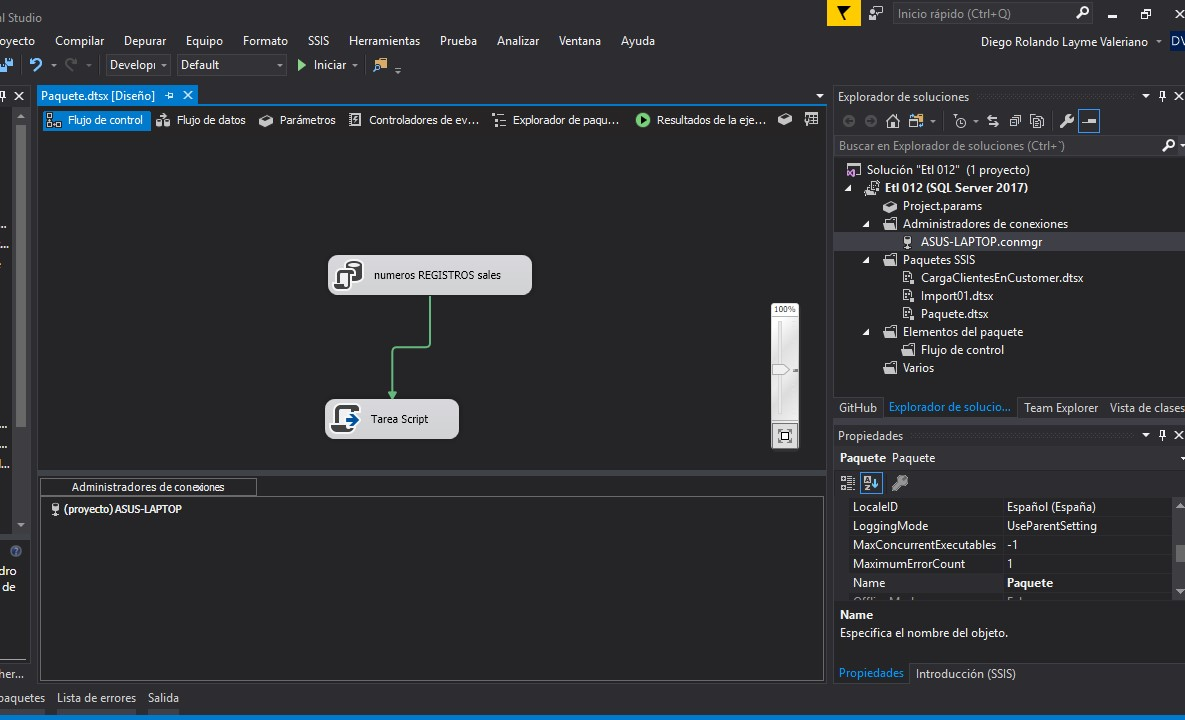
\includegraphics[width=10cm]{imagenes/registros_componentes.jpg}
        \end{center}
        
        
                
    \item Abrimos la Tarea de Ejecutar SQL y configuramos la consulta para obtener la cantidad de registros en SQL Statement
     \begin{center}
            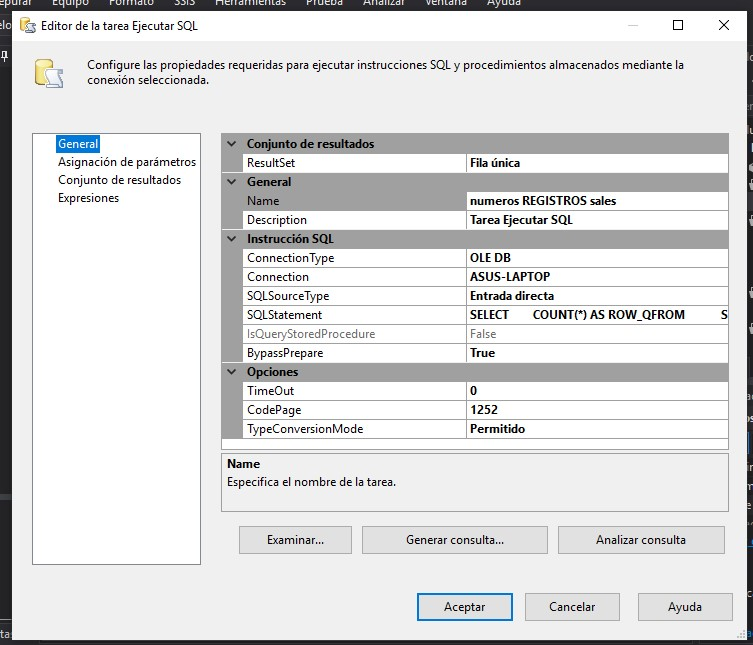
\includegraphics[width=10cm]{imagenes/registros_flujo_configuracion.jpg}
        \end{center}
        
        
                
    \item Asignar la variable en “Numero de Registros Sales”
     \begin{center}
            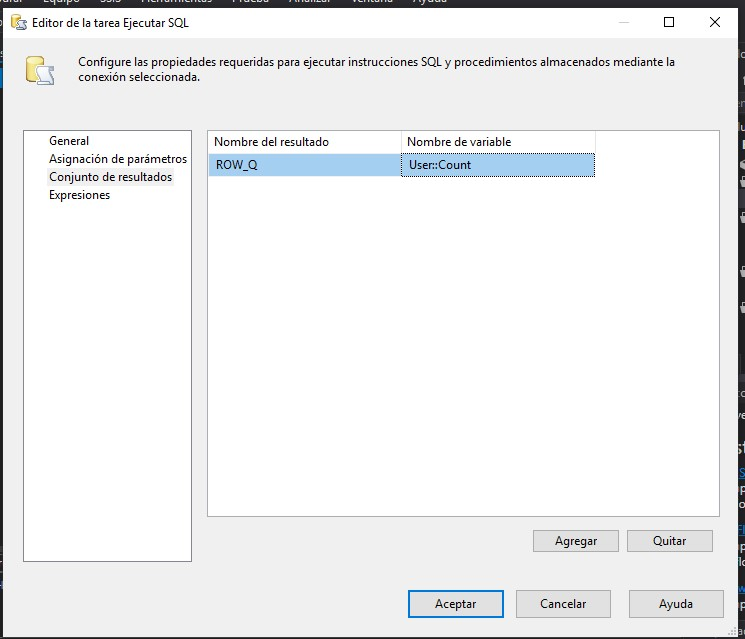
\includegraphics[width=10cm]{imagenes/registros_result_set.jpg}
        \end{center}
        
    \item Editamos el componente Tarea Ejecutar SQL
     \begin{center}
            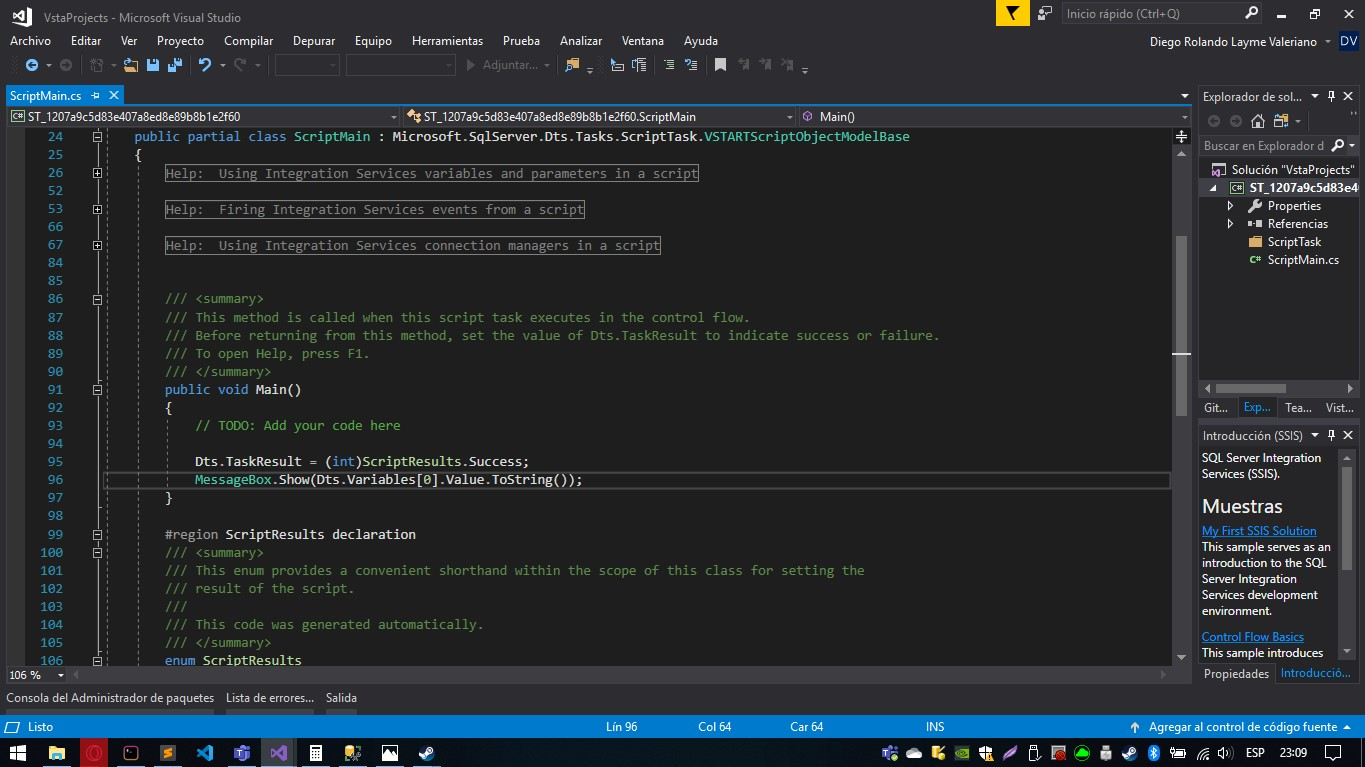
\includegraphics[width=10cm]{imagenes/registros_proyecto_print.jpg}
        \end{center}
        
    \item Finalmente Ejecutamos
     \begin{center}
            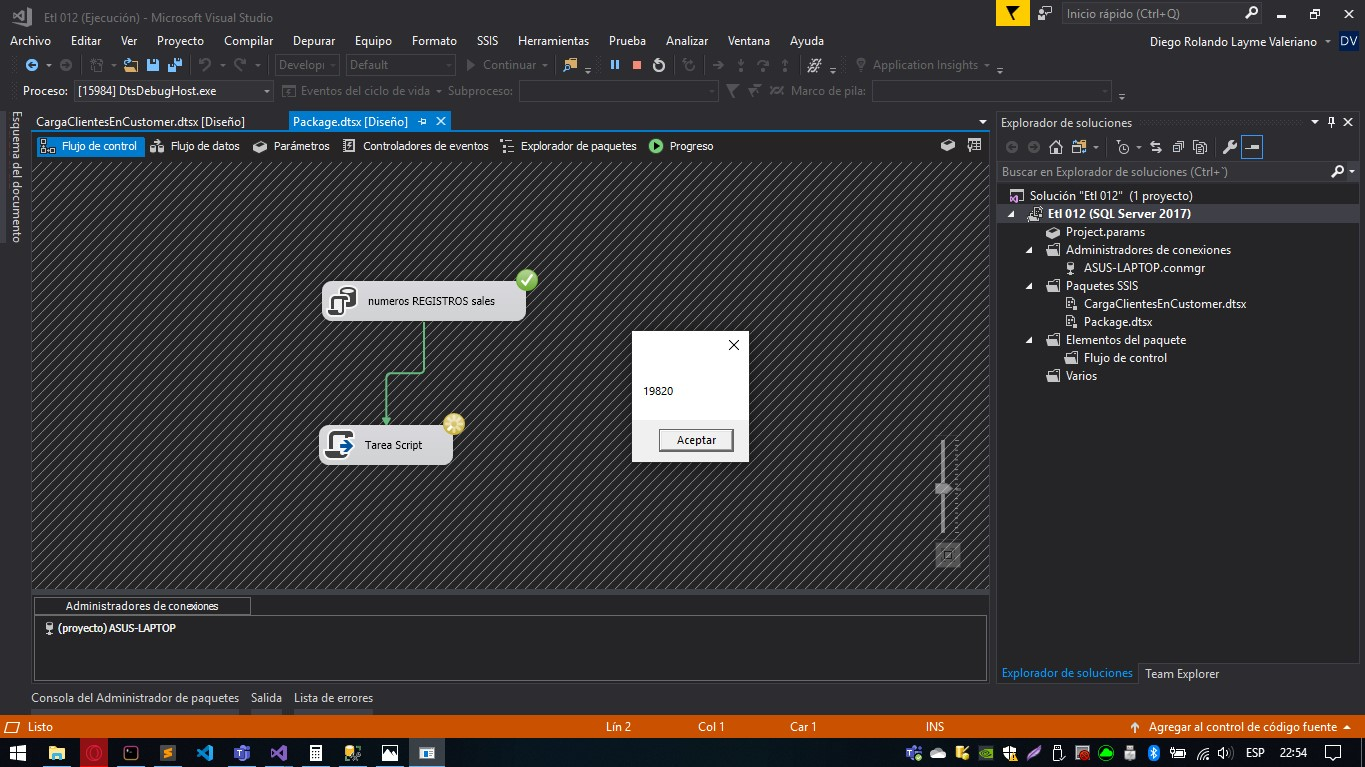
\includegraphics[width=10cm]{imagenes/registros_final.jpg}
        \end{center}
\end{enumerate}